\documentclass{article}
\usepackage[margin=1in]{geometry}
\usepackage{hyperref}
\usepackage{graphicx}
\usepackage{fancyvrb}


\newcommand{\myitem}{\paragraph}
\begin{document}

\myitem{CSCI 342, Fall 2017, Homework \# 4}

\myitem{Due date:}  Friday, November 10, midnight.  ZIP all files
together.

\myitem{Instructions:}


This assignment tests your understanding of JavaScript and its
interaction with HTML user interfaces.  You must match the appearance
and behavior of the following web page:

\centerline{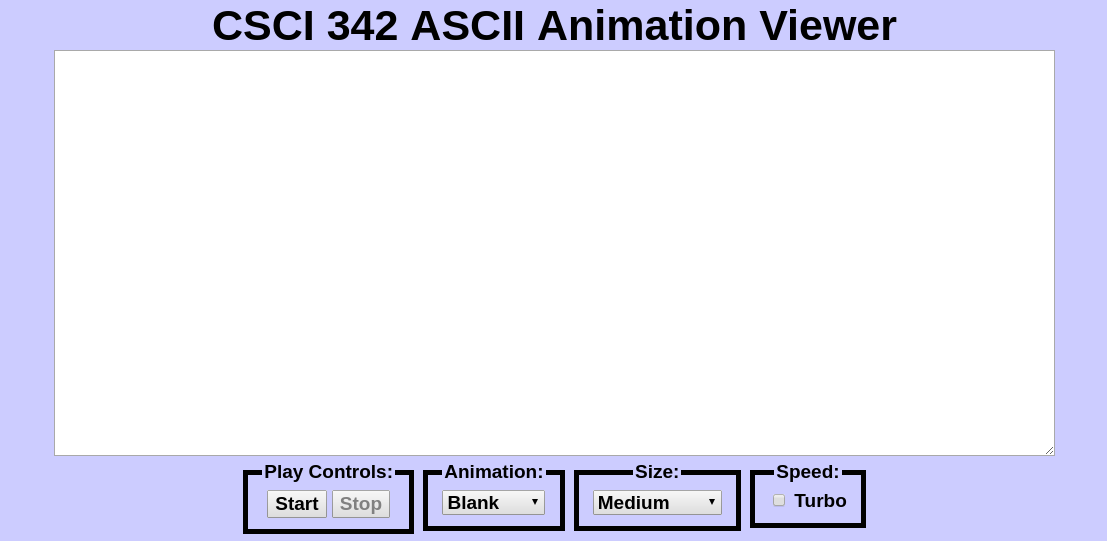
\includegraphics[scale=0.5]{images/screenshot.png}}

ASCII art is pictures that consist of text characters.  ASCII art has
a long history as a way to draw pictures for text-only monitors or
printers.  We will draw animated ASCII art, or "ASCIImation." You can
see a number of examples on the webpage
\url{http://www.asciimator.net/} Groups of nerds are working to
recreate the entire movies Star Wars and The Matrix as ASCIImation.

The first task is to create a page {\tt ascii.html} with a user
interface (UI) for creating/viewing ASCIImations.  No skeleton files
are provided.  Your page should link to a style sheet you'll write
named {\tt ascii.css} for styling the page.  After creating your page,
you must make the UI interactive by writing JavaScript code in {\tt
  ascii.js} so that clicking the UI controls causes appropriate
behavior.  Your HTML page should link to your JS file in a script tag.

You should also create an ASCIImation of your own, stored in a file
named myanimation.txt.  Your ASCIImation must show non-trivial effort,
must have multiple frames of animation, and must be entirely your own
work.  Be creative!

In total you will turn in the following
files:
\begin{itemize}
\item {\tt ascii.html}, your web page
\item {\tt ascii.css}, the style sheet for your
  web page
\item {\tt ascii.js}, the JavaScript code for your web page
\item {\tt myanimation.txt}, your custom ASCII animation as a plain text file
\item {\tt myanimation.js}, your custom ASCII animation as JavaScript code
\end{itemize}
Please ZIP them all together for submission.

\myitem{Appearance Details:}
\begin{itemize}
\item
  The page should have a title of
  ASCIImation.
\item
  Your page must link to the JavaScript and CSS resources:
\begin{itemize}
  \item
 {\tt animations.js} for the standard animations.  This file is
 available on the homework page.
\item
  {\tt myanimation.js} (you will write this file)
\item {\tt ascii.js} (you will write
  this file)
\item {\tt ascii.css} (you will write this file)
\end{itemize}
\item
 The overall page has a background color of
{\tt \#CCCCFF}. The preferred font for all text on the page is the default
sans-serif font available on the system, in size 14pt, in bold.
\item
The
top of the page contains a heading in 32pt bold text, centered
horizontally within the page. There is no margin between the heading
content area and other neighboring content on the page.
\item
Under the
page's heading is a text box with 80 columns and 20 rows, centered
horizontally.  Its width is 90\% of the page size and height is 400px.
It uses a 12pt bold monospace font initially.  CSS width/height
properties will set the text box's size, but you must put rows/cols
attributes in your textarea HTML element for the page to validate.
\item
Below the text box is a set of controls grouped into several field
sets, each with a 5px black border around it and a label on top.
Their behavior is described below.  To get the field sets to appear in
a row horizontally, see textbook Chapter 4's section about Element
Visibility and the display property.  You should make sure that the
tops of the field sets line up by setting their vertical alignment.
The text area and control field sets are centered horizontally.
\end{itemize}

\myitem{Behavior Details:} The following are the groups of controls at
the bottom of the page and each control's behavior.  Although
we put controls in a {\tt form} in past assignments, do not use a {\tt form}
tag on your page this time.  All interactivity will be handled with
javascript and there will be no {\tt Submit} button.

\begin{description}
\item[Play Controls:]\mbox{}
  \begin{description}
\item[Start:] When clicked, animation begins.  When the page is idle,
  all frames of the animation are visible.  Frames are separated by 5
  equals signs and a line break (\verb|\n|) character.  When
  animation starts, whatever text is currently in the text box is
  broken apart to produce frames of animation.  This might be a
  pre-set animation, or text that the user has typed manually.  During
  animation, one frame is visible at any moment, starting with the
  first frame.  By default, the animation changes frames once every
  250ms.  When the animation reaches the last frame, it loops back
  around and repeats indefinitely.  (You must implement your animation
  using a JavaScript timer with the setInterval function.)
\item[Stop:] When clicked, halts any animation in progress.  When animation is stopped, the text that was in the box before animation began is returned to the box.
\end{description}
\item[Animation:] A drop-down list of ASCII animations. When one of
  the animations is chosen (onchange), the main text area updates to
  display all text of the chosen animation. The choices available are:
  Blank, Exercise, Juggler, Bike, Dive, Custom.  Initially the Blank
  animation is selected and no text is showing in the text entry box.
  Your {\tt ascii.html} page should link to a provided file {\tt
    animations.js} that declares the ASCIImations as global string
  variables named {\tt EXERCISE}, {\tt JUGGLER}, {\tt BIKE}, and {\tt
    DIVE}. You shouldn't edit this file, but your {\tt ascii.js} file
  can refer to these variables. For example, if you have a textarea on
  your page with an id of mytextarea:
  \verb|$("mytextarea").value = JUGGLER;|

The provided {\tt animations.js} file also defines a global
associative array named ANIMATIONS that maps from indexes (keys) that
are strings equal to the names of the animations, such as ``Bike'' or
``Exercise'', to values that are long strings representing the entire
animation text for that image.  Using this array well can help you
avoid redundancy.  Here is a short example that uses the ANIMATIONS
array:
\begin{Verbatim}[frame=single]
var whichOne = "Juggler"; 
$("mytextarea").value = ANIMATIONS[whichOne];
\end{Verbatim}

The user may type new text in the field after choosing a pre-set
animation.  The animation shown when Play is pressed should reflect
these changes.  (i.e., Don't capture the text to animate until the
user presses the Start button.)  You may assume that the user will not
try to type into the text area while animation is in progress.  You
may also assume that the user will not use the selection box to change
to a new animation while animation is occurring; assume that the user
will stop any existing animation before changing to a new one.

\item[Custom Animation:] The Custom choice in the Animation box should
  show an animation that you have created.  The file {\tt stringmaker.html}
    converts your animation to a string you can put into
  {\tt myanimation.js}.

  Don't put comments or headings in {\tt myanimation.txt;} it should
  NOT be encoded by StringMaker.  The text file contains your
  animation in plain text, so that if someone did Select All, Copy,
  and Paste into your ASCIImation page, it would animate properly.
  You are turning in your custom animation in two ways: once as a
  plain {\tt .txt} file, and in a {\tt .js} file as an encoded string.

\item[Font Size:] A drop-down list of font sizes. When one of the font
  sizes is chosen, it immediately sets the font size in the main text
  area.  The font sizes listed in the drop-down list, and the
  corresponding font size to set, are: Tiny (7pt), Small (10pt),
  Medium (12pt), Large (16pt), Extra Large (24pt), XXL (32pt)

  Initially Medium is selected and the text is 12pt in size. If the
  animation is playing and one of these buttons is clicked, the font
  size changes immediately.  Note that when you write the code for
  changing the font sizes, it is easy to introduce redundancy.  By
  setting a value attribute on each of the options in the drop-down
  list, you can avoid a long series of if/else statements.

\item[Speed:] Contains a single checkbox labeled "Turbo".  When the
  box (or the text next to it) is clicked, causing the box to become
  checked, it sets the speed of animation to use a 50ms delay instead
  of 250ms.  When unchecked, the speed goes back to 250ms.  Initially
  the box is unchecked and the delay is 250ms.  If the animation is
  playing and the box is checked/unchecked, the change should take
  effect immediately (the user shouldn't have to stop and restart the
  animation to see the change).  Checking the box shouldn't cause the
  animation to start if it wasn't already started.  It also shouldn't
  reset what frame is showing; it should just change the delay.

\item[Control Enabling/Disabling:] Modify your GUI to disable
elements that the user shouldn't be able to click at a given time.
Initially and whenever animation is not in progress, the {\bf Stop} button
should be disabled.  When animation is in progress, {\bf Start} and the
select box of animations should be disabled.  The {\bf Size} box and
{\bf Turbo}
checkbox should always be enabled.  Enable or disable a control with
its disabled property.  For example, to disable a control with id of
customerlist:
\begin{Verbatim}[frame=single]
  document.getElementById("customerlist").disabled = true;
\end{Verbatim}

\end{description}

\myitem{Development strategy:}
\begin{enumerate}
  \item Write the basic HTML content
    including the proper UI controls.  (Don't use the form tag.)
  \item
    Write
    your CSS code to achieve the proper layout.
  \item
    Write a small amount
of "starter" JS code and make sure that it runs.  (For example, make
it so that when the Start button is clicked, an alert box appears.)
\item
  Implement code to change the animation text and font sizes.  Make
it so that when an option is chosen in the selection box, the proper
text string appears in the text area.  Get the font size options
working.
\item
  Implement a minimal Start behavior so that when Start is
clicked, a single frame of animation is shown. Clicking Start multiple
times would show successive frames of animation.

\item Use {\tt setInterval}
to implement the proper animation based on your previous code.
\end{enumerate}

\myitem{Debugging:}

\begin{itemize}
\item
We strongly recommend that you use debugging tools
such as the one builtin to Chrome.  
\item
JSLint (\url{www.jslint.com}) can
help you find common JavaScript bugs.  Since this is your first
JavaScript program, you will probably encounter tricky bugs.  If so,
paste your code into JSLint to look for possible errors or warnings.
\item
  For full credit, your {\tt .js} file must be written in JavaScript "strict"
mode by putting this exact line of code at the top:
\begin{Verbatim}[frame=single]
  "use strict";
  \end{Verbatim}
\end{itemize}

\myitem{Implementation and Grading:}
\begin{itemize}
\item
You can use jQuery or Vanilla javascript.
\item
Express all stylistic information on the page in CSS using your style
sheet file.  For full credit, your style sheet must successfully pass
the W3C CSS validator.  You should not use HTML or CSS constructs that
have not been discussed in lecture, slides, or textbook chapters
during the first five weeks of the course.  
\item
Format your HTML, CSS, and JS to be readable, like to the examples in
class. Place a comment header atop each HTML/CSS/JS file.  Your
JavaScript should have more descriptive comments, including a header
on each function and complex sections of code describing the relevant
code, the function's behavior, {\em etc.}
\item
For full credit, your JavaScript code should pass the provided JSLint
tool with no errors reported (warnings OK).  You should follow
reasonable style guidelines similar to those of all your programming
classes.  In particular, avoid redundant code, and use parameters and
return values properly.
\item
Minimize the use of global variables.  Do not store DOM element
objects, such as those returned by the document.getElementById
function, as global variables unless you need to.
\item
Format your code similarly to the examples from class.  Properly use
whitespace and indentation.  In your HTML, do not place more than one
block element on a line or begin a block element past the 100th
character.  In your JavaScript, properly space/indent your code, and
do not write any lines of code longer than 100 characters.
\end{itemize}


\paragraph{Acknowledgements:} This assignment
 is adapted from one that is:
Copyright \copyright Marty Stepp / Jessica Miller, licensed under
\href
    {https://creativecommons.org/licenses/by/2.5/}
    {Creative Commons Attribution 2.5 License}.
    All rights reserved.
Special
thanks to Dave Reed of Creighton University for the original idea of
this assignment.





\end{document}
